%(BEGIN_QUESTION)
% Copyright 2006, Tony R. Kuphaldt, released under the Creative Commons Attribution License (v 1.0)
% This means you may do almost anything with this work of mine, so long as you give me proper credit

Energi kreves for å komprimere eller strekke en mekanisk fjær, fordi en kraft virker over en parallell forflytning. Beregning av arbeidet som utføres ved komprimering eller strekk av en fjær er mer komplisert enn beregning av arbeid ved løfting av en vekt, fordi kraften ($F$) ikke er konstant. De fleste fjærer har over korte avstander en lineær sammenheng mellom kraft og forflytning (komprimert eller strukket lengde), kjent som {\it Hookes lov}:

$$F = kx$$

\noindent
Der,

$F$ = Kraften som kreves for å komprimere eller strekke en fjær med avstanden $x$, i pund (lb) eller newton (N)

$x$ = Avstanden fjæren komprimeres eller strekkes, i fot (ft) eller meter (m)

$k$ = Fjærkonstanten, i pund per fot (lb/ft) eller newton per meter (N/m)

\vskip 10pt

Fjærbaserte vekter utnytter dette linearitetsprinsippet: dobbel vekt på fjærvekten gir dobbelt nåleutslag på en lineær skala.

For å beregne hvor mye {\it arbeid} som utføres ved komprimering eller strekk av en fjær, må vi ta hensyn til at kraften {\it ikke} er konstant når fjæren deformeres. Her er graf av kraft mot forflytning et nyttig verktøy for å beregne arbeid.

Tegn grafen for kraften som kreves for å komprimere en fjær med konstant 60 pund per fot, og beregn deretter arbeidet som kreves for å komprimere den 3 fot:

$$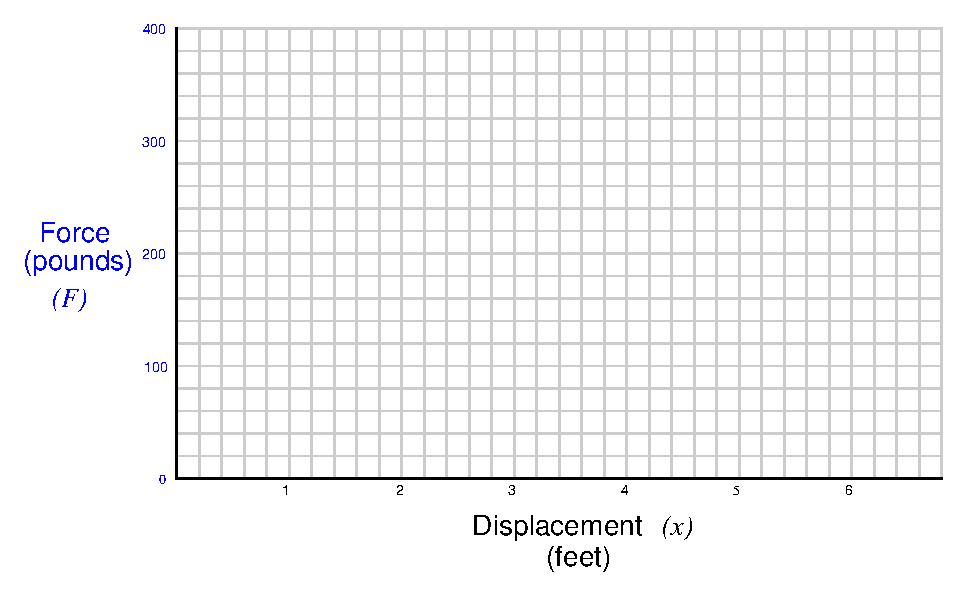
\includegraphics[width=15.5cm]{i01575x01.eps}$$

\vskip 20pt \vbox{\hrule \hbox{\strut \vrule{} {\bf Forslag til sokratisk diskusjon} \vrule} \hrule}

\begin{itemize}
\item{} I hvilken ende av fjærens bevegelse (0 fot strekk eller 3 fot strekk) lagrer fjæren mest energi {\it per tomme} ekstra strekk?
\item{} Hvis du skulle tegne en graf over lagret energi per tomme fjærbevegelse, hvilken form ville grafen få?
\item{} Identifiser matematisk fortegn (positivt eller negativt) for kraft ($F$), differensial av avstand ($dx$) og arbeid ($W$) mens fjæren {\it belastes} av en ytre kraft.
\item{} Identifiser matematisk fortegn (positivt eller negativt) for kraft ($F$), differensial av avstand ($dx$) og arbeid ($W$) mens fjæren {\it avlastes} mot sin hvilestilling.
\item{} Anta at denne fjæren sitter i en pneumatisk reguleringsventil som åpner ved lufttilførsel (air-to-open). Hvis reguleringssløyfen oscillerer og ventilspindelen dermed beveger seg opp og ned periodisk, hva representerer da beregnet arbeid ved fjærkompresjon i form av trykkluftforbruk? Er denne arbeidsmengden viktig for oss, eller bare akademisk?
\item{} Anta at en air-to-open pneumatisk reguleringsventil sykler $\pm$10\% nær helt stengt posisjon. Anta så at samme ventil sykler $\pm$10\% nær helt åpen posisjon. I hvilken situasjon forbruker ventilen mest trykkluft per tidsenhet? Forklar hvorfor.
\end{itemize}

\underbar{file i01575}
%(END_QUESTION)





%(BEGIN_ANSWER)

$$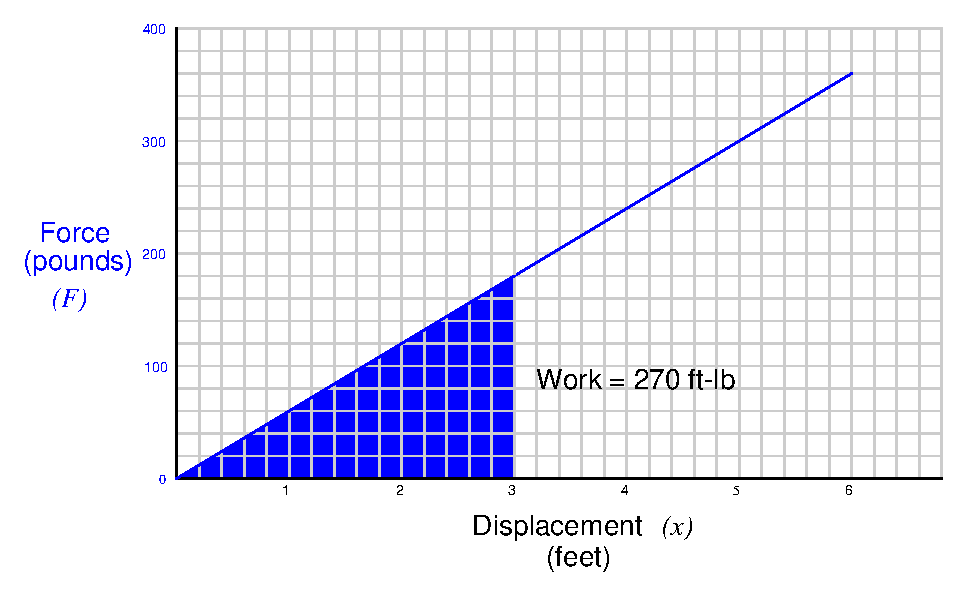
\includegraphics[width=15.5cm]{i01575x02.eps}$$

%(END_ANSWER)





%(BEGIN_NOTES)

Husk at arealet av en trekant er grunnlinje multiplisert med høyde, delt på 2.

\vskip 10pt

Vi kan også løse denne oppgaven med litt kalkulus:

$$W = \int_0^3 F \> dx \hbox{\hskip 50pt} F = kx$$

$$W = \int_0^3 kx \> dx$$

$$W = \int_0^3 60x \> dx$$

$$W = 60 \int_0^3 x \> dx$$

$$W = 60 \left[ {1 \over 2}x^2 \right]_0^3$$

$$W = 60 \left[ {3^2 \over 2} - {0^2 \over 2} \right]$$

$$W = 60 \left[ 4.5 - 0 \right]$$

$$W = 60 \left[ 4.5 \right]$$

$$W = 270 \hbox{ ft} \cdot \hbox{lb}$$

%INDEX% Mathematics, calculus: integral (work)

%(END_NOTES)
